\documentclass{article}
\usepackage[preprint,eandd]{neurips_2026}
\usepackage[utf8]{inputenc}
\usepackage[T1]{fontenc}
\usepackage{amsmath}
\usepackage{amssymb}
\usepackage{booktabs}
\usepackage{graphicx}
\usepackage{hyperref}
\usepackage[all]{hypcap}
\usepackage{microtype}
\usepackage{url}
\usepackage{xurl}
\usepackage{xcolor}
\providecommand{\Description}[1]{}
\makeatletter
\setlength{\@fptop}{0pt}
\setlength{\@fpsep}{16pt}
\makeatother
\hypersetup{
  hidelinks,
  pdftitle={DFAH-Bench: Benchmarking Observable Agent Instability in Financial Decision-Making},
  pdfauthor={Raffi Khatchadourian},
  pdfsubject={Replay measurement for observable financial-agent execution},
  pdfkeywords={AI agents, financial AI, replay, tool use, benchmark evaluation}
}

\newcommand{\dar}{\mathrm{DAR}}
\newcommand{\tar}{\mathrm{TAR}}
\newcommand{\tarseq}{\mathrm{TAR}_{\mathrm{seq}}}
\newcommand{\tarbag}{\mathrm{TAR}_{\mathrm{bag}}}
\newcommand{\tarset}{\mathrm{TAR}_{\mathrm{set}}}
\newcommand{\tarstrong}{\mathrm{TAR}_{\mathrm{strong}}}
\newcommand{\gapmetric}{\Delta_{\mathrm{DT}}}

\begin{document}

\title{DFAH-Bench: Benchmarking Observable Agent Instability\\in Financial Decision-Making}

\author{
  Raffi Khatchadourian \\
  IBM Financial Services Market \\
  New York, NY, USA \\
  \texttt{raffi.khatchadourian1@ibm.com}
}

\maketitle

\begin{abstract}
A financial agent can repeat a decision while changing the work behind it.
DFAH-Bench operationalizes the Determinism--Faithfulness Assurance Harness
(DFAH), pairing decision agreement with tool-path agreement on the same
qualified replays, then extends that qualification principle to evidence,
authorization, execution and task outcomes.
Retrospective and prospective replay analyses expose process variation behind
stable decisions. Across 570 eligible prospective episodes, decision agreement
is 94.2--95.1\%, while agreement on ordered tools, arguments and results is
45.0--51.5\%; one stratum falls one group below its prespecified coverage
minimum. A separate capture diagnostic shows that systematic omissions can
preserve perfect replay agreement.
Using the $\tau$-Knowledge banking environment, we retain 1,080 scheduled
episodes and 1,033 known native outcomes across separate cohorts with
open-weight and frontier generators. Missing outcomes prevented the planned
tests, so comparisons are descriptive. On the primary schedule, structural
checks alone yield more successes than either
gate-and-recovery bundle. The typed-choice
bundle has lower mean episode cost than the generative bundle on complete task
pairs, but produces fewer successes under every assignment of unknown outcomes.
Input limits and recovery behavior materially shape these results.
Fixed-state probes reveal higher decision agreement alongside lower agreement
with constructed policy labels, and separately expose sensitivity to retained
generator rationale in a selected authorization case. Together, the findings
connect replay observability to evidence,
authorization, completion and cost: evidence sufficiency needs direct assessment
alongside repeatability.
\end{abstract}

\begin{center}
\textbf{Code and public artifacts:}
\url{https://github.com/ibm-client-engineering/output-drift-financial-llms}
\end{center}

\section{Introduction}

This work grew out of my own use of frontier and open-weight models and their
tools. Their rapid development raised a persistent concern: how to track what
an agent actually does as models, tools, and permissions change. In regulated
industries, adoption depends on the controls and evidence behind an action.

An AI coding agent searched beyond its repository boundary, materializing
cloud-drive placeholders locally and triggering a security alert. The search returned no
file match or document content, and the reviewed records contained no
affirmative evidence that file contents were externally shared or transmitted
to the model. An email-connected assistant separately treated a drafting
request as permission to send before review and added unsupported personal details.

These experiences motivate our experiments on observable execution in synthetic
financial tasks: what changes when an agent repeats a task under fixed settings?

Financial agents retrieve context, apply controls, inspect records, and modify
state. Task-specific authorization must govern their data access and actions,
even when connected tools are authenticated.

Two runs may both return \emph{escalate}, while one checks sanctions and
customer history and the other jumps directly to a risk score. A final-label
metric treats them as equivalent. Operational review distinguishes optional
tools, provider-dependent behavior, and inconsistently executed controls
according to the workflow's requirements.

DFAH-Bench asks whether the observable work behind a decision survives replay:

\begin{itemize}
  \item \textbf{RQ1:} How often do decisions and tool paths agree across
  identical financial-agent replays?
  \item \textbf{RQ2:} When the decision is stable, how much process variation
  remains hidden from an outcome-only score?
\end{itemize}

The benchmark contributes:

\begin{itemize}
  \item a replay-eligibility protocol that pairs
  closed decisions with tool paths, aligns their denominators, and distinguishes
  an observed empty path from a missing required channel;
  \item a configuration-level analysis over 4,157 retained episodes from configurations with observed tool use that
  separates controlled from provider-default evidence and decomposes variation
  into tool order, multiplicity, and distinct-name changes, together with
  separate argument-aware local and prospective API extensions;
  \item a separate local capture diagnostic showing how systematically omitted
  calls can preserve perfect replay agreement;
  \item a banking intervention study that measures evidence, permission,
  execution, native task completion and API cost under a shared qualification
  contract, with separate primary and exploratory cohorts; and
  \item an instrumentation blueprint for recording provenance, evidence
  confidence, freshness and promotion decisions.
\end{itemize}

DFAH qualifies comparability and required channels before pairing decision and
path agreement over the same retained episodes. Observability is part of the estimand.

The headline blind spot is concrete: unanimous decisions can conceal varying
paths.  In the complete-coverage Gemini 2.0 Flash row, 24.7\% of
unanimous-decision groups changed tool sequence.  A separate prospective API
extension points the same way under argument-aware capture, with
25.8--27.3-point decision--path gaps across 190 eligible groups.

The benchmark is diagnostic: it identifies changes for inspection alongside
separate assessments of task quality, fairness, and policy compliance.
The banking intervention asks what happens when a recorded judgment becomes
a condition for execution. Distinguishing input admission, model assessment,
permission, dispatch and outcome shows where a control acts and where the
workflow stops.

\section{Related Work and Positioning}

\paragraph{Financial evaluation.}
FinBen measures financial language-model capabilities across many tasks
\citep{xie2024finben}.  FinAgentBench evaluates multi-step retrieval in finance
\citep{choi2025finagentbench}, while FinResearchBench uses logic trees and an
agent judge for financial research reports~\citep{sun2025finresearchbench}.
FinTrace evaluates expert-annotated financial trajectories for action
correctness, efficiency, process quality, and output quality
\citep{cao2026fintrace}. DFAH complements these quality measures by asking
whether a fixed configuration repeats the same case the same way.

\paragraph{Tool agents and trajectories.}
$\tau$-bench introduced repeated-trial \(\mathrm{pass}^k\) for interactive
tool agents~\citep{yao2024taubench}; ToolSandbox evaluates intermediate stateful
milestones~\citep{lu2025toolsandbox}.  TRAJECT-Bench scores tool selection,
arguments, and ordering against reference paths~\citep{he2026traject}. DFAH
compares paths across replays of the \emph{same} case and configuration.

\paragraph{Anchor sensitivity.}
A natural replay baseline matches each decision and ordered tool-name sequence
to the first replay. DFAH-Bench uses modal agreement over qualified groups,
pairs decision agreement (DAR) and tool-path agreement (TAR) on the same
denominator, task-weights cases, and separates
sequence, multiset, and set variation. Retrospective logs support tool-name
comparison; argument-aware capture is prospective. Modal agreement is by
construction at least first-anchored agreement.
The difference---2.3--5.3 points across the four API configurations and up to
12.7 points for one eight-replay local configuration---quantifies the estimand
change.

\paragraph{Repeated outputs and observability.}
Self-consistency uses diverse reasoning samples to improve answers
\citep{wang2023selfconsistency}; ReasonBENCH studies multi-run variation in
reasoning quality and cost~\citep{potamitis2025reasonbench}.  Finance and
accounting outputs also show material repeat variation at scale
\citep{wang2025consistency}. Faithfulness in model-explanation research concerns whether an
explanation reflects the process producing a prediction~\citep{jacovi2020faithfulness}.
The replay metrics here quantify agreement among recorded decisions and paths;
the capture diagnostic separately compares records with dispatched operations.
Both support visibility into agent behavior~\citep{chan2024visibility}.
Every Eval Ever standardizes aggregate and instance-level evaluation records
across harnesses, including agentic tool-call traces~\citep{batzner2026every}.
DFAH qualifies replay measurements that such schemas can report.
Runtime-governance systems control what a financial agent may
do~\citep{szpruch2026runtime}; DFAH-Bench measures whether a fixed
configuration repeats what it observably did.

\section{Benchmark Design}

\subsection{Tasks and replay unit}

Each case fixes the prompt, tool schemas, tool implementation, and synthetic
data.  A configuration is the model identifier together with provider,
sampling controls, harness, and tool interface.  A \emph{case group} is the
set of repeated episodes for one case and configuration.

The retrospective and prospective API studies use the first two workflows in
Table~\ref{tab:tasks}; the bounded local harness check uses the third.  Cases
were programmatically authored to exercise intended control branches; they
contain no customer or transaction data.  Their provisional labels define the
decision space; evaluating financial accuracy would require independent expert
adjudication.  A portfolio development
fixture was excluded before this analysis after a
fixture review found inconsistencies between its declared total, runtime tool
arithmetic, and several reference rationales.  All reported analyses use the
remaining fixtures.

\begin{table}[t]
\caption{Synthetic workflows used across the three original replay studies.
The separate eight-case capture diagnostic is described in
Section~\ref{sec:capture-diagnostic}.}
\label{tab:tasks}
\centering
\small
\begin{tabular}{@{}p{0.19\columnwidth}p{0.35\columnwidth}p{0.36\columnwidth}@{}}
\toprule
Task & Decision ontology & Example observable tools \\
\midrule
Compliance (50) & dismiss / investigate / escalate & sanctions, customer profile, risk score \\
Financial DataOps (50) & auto-fix / escalate / quarantine & exception details, reference data, validation \\
Local reconciliation (50) & reconcile / investigate / escalate & internal record, external record, policy, variance \\
\bottomrule
\end{tabular}
\end{table}

\subsection{Agreement measures}

For case \(c\), let \(N_c\) repeated episodes produce decisions \(d_{cr}\) and
ordered tool-name paths \(t_{cr}\).  The empty sequence is retained when an
episode calls no tool.  Every retained compact log explicitly captured the
trajectory field; a missing, null, malformed, or structurally inconsistent
required trajectory would make the replay group ineligible rather than enter
the metric as an empty path.  Channel availability and tool activity are
therefore distinct.  Decision and sequence-level trajectory agreement are modal
fractions:

\begin{align}
\dar_c &= \max_y \frac{1}{N_c}\sum_{r=1}^{N_c}\mathbf{1}[d_{cr}=y], \\
\mathrm{TAR}_{\mathrm{seq},c} &= \max_t \frac{1}{N_c}\sum_{r=1}^{N_c}\mathbf{1}[t_{cr}=t], \\
\Delta_{\mathrm{DT},c} &= \dar_c-\mathrm{TAR}_{\mathrm{seq},c}.
\end{align}

DAR quantifies decision repeatability.  Recorded-path repeatability is measured by
\(\tarseq\) for ordered tool names and, in prospective captures,
\(\tarstrong\) for ordered names, canonical arguments, and deterministic result
hashes.  Both are scored only for eligible groups whose fixed configuration and
required channels are present.  Capture fidelity asks whether those records
preserve executed operations; Section~\ref{sec:capture-diagnostic} examines
that relationship through controlled record omissions.

In DFAH, faithfulness denotes replay fidelity of the recorded execution path:
\(\tarseq\) and \(\tarstrong\) measure that fidelity at the path boundary,
while explanation faithfulness and answer correctness are separate constructs.

The gap is paired within a case.  A positive \(\gapmetric\) means decisions
agree more often than observable paths, so an outcome-only score hides route
variation.  Zero means the two agreement rates align.  A negative value means the path is more concentrated than the
separately modal decision; this is possible because DAR and TAR choose their
modes independently.  Accordingly, \(\gapmetric\) is a paired contrast between
marginal concentrations.  RQ2 supplies
the direct same-decision test by conditioning on groups with unanimous
decisions and asking whether more than one path remains.  There is no universal
cutoff.  A workflow should
pre-register its own investigation trigger based on consequences and replay
count---for example, a unanimous decision with multiple paths or a positive gap
that persists under the frozen sensitivity analysis.  The useful question is
what changed and whether a required check disappeared.

Sequence equality distinguishes call order and multiplicity, but the legacy
logs omit arguments and results.  A tool name also hides scope: searches
bounded to a project and a home directory share a name, schema, and call count,
but not a data-access surface.  Name-only TAR scores them identically;
argument-aware capture separates them.  In prospective captures, \(\tarstrong\)
applies the same modal calculation to ordered tool names, canonical arguments,
and deterministic result hashes; it cannot recover omissions from the
retrospective logs.
Canonical arguments are strict JSON encoded as UTF-8 with sorted object keys
and compact separators; non-JSON and non-finite values are rejected before
SHA-256 hashing.  This preserves type and array-order differences while
removing object-key and whitespace variation.  We
therefore add two construct sensitivities: \(\tarbag\) canonicalizes each path as a multiset,
retaining repeated calls while ignoring order; \(\tarset\) retains only distinct
tool names.  Set equality is a coarse contact proxy.  Assessing the consequences
of reordered or repeated controls requires the workflow's policy and state.

Exact equality is deliberately conservative.  Text-similarity measures encode
different lexical, statistical, and semantic constructs, and their suitability
depends on the application~\citep{li2026similarity}.  A future semantic
trajectory score could complement exact TAR, but it would change the estimand
and would need finance-specific validation before near-matches were treated as
operationally equivalent.

\section{Experimental Setup}

The complete retained ledger contains 5,501 episodes in 887 case groups from
ten recorded configurations.  Primary tool-path analysis requires at least one
observed tool call in the configuration.  Two configurations in the
retrospective corpus produced no tool calls across 1,344 episodes in 168 groups;
their logs remain in
the lineage record but are excluded from the primary slice.  This is an
eligibility decision about those recorded configuration--harness combinations.  The
required-channel check found no missing or malformed trajectory fields in this
scope, so it excluded zero additional groups; the zero-tool exclusion concerns
observed activity.  This configuration-level rule was adopted
during the post-run corpus audit.  Retaining the zero-tool
rows leaves the 122 varying groups unchanged but changes the pooled rate from
122 of 627 (19.5\%) to 122 of 791 (15.4\%); configuration-specific results are
unchanged.  Prompt-visible tool outputs are
deterministic functions of fixed fixture data and supplied arguments; timestamps
used in DataOps side-effect bookkeeping are not returned to the agent.
The
resulting primary slice in \autoref{tab:protocol-coverage} contains 4,157 episodes
in 719 groups across eight configurations.  Local configurations have eight repeats per available case at
temperature zero and seed 42.  Gemini configurations have three repeats at
temperature zero without a provider seed.  Claude configurations have three
repeats without a provider seed; a legacy runner omitted the requested
temperature, so those calls used the provider default even though retained
log fields said zero.  We correct that description here and treat Claude only
as a sensitivity set.  The exact evaluated object is therefore a deployment
configuration, including its provider and harness.

Two reported configurations have incomplete coverage.  Gemini 2.5 Pro has 44
compliance groups and Claude Opus 4 has 75 groups.  These slices are contiguous
prefixes: compliance cases 1--44 for Gemini Pro and DataOps 1--25 for Opus.
The logs leave the cause unresolved; analysis is restricted to those observed
prefixes.  DeepSeek pilot episodes are
omitted because only two cases completed.

\begin{table*}[t]
\caption{Replay evidence map. Fractions give eligible over scheduled groups or
episodes.  The retrospective core includes 600 complete-coverage groups and 119
groups from two contiguous prefixes.}
\label{tab:protocol-coverage}
\centering
\scriptsize
\setlength{\tabcolsep}{3.5pt}
\begin{tabular}{@{}lrrrrp{0.24\textwidth}p{0.20\textwidth}@{}}
\toprule
Study & Cfg. & Groups & Episodes & Replays & Observable & Role \\
\midrule
Retrospective core & 8 & 719 & 4,157 & 3 or 8 & decision + ordered tool names & primary analysis \\
Prospective API extension & 2 & 190/200 & 570/600 & 3 & names + arguments + result hashes & version-pinned evidence \\
Local harness check & 2 & 99/100 & 792/800 & 8 & fixed four-tool strong path & capture verification \\
Local capture diagnostic & 2 & 16/16 & 48/48 & 3 & names + arguments + result hashes & paired capture-loss diagnostic \\
\bottomrule
\end{tabular}
\end{table*}

We first average case measures within each task and then weight available tasks
equally for each configuration.  Reported ranges are finite-corpus
case-resampling sensitivity intervals based on 5,000 within-task resamples.
They assess sensitivity to the composition of the observed authored cases under
exchangeable reweighting and remain conditional on the observed cases and repeats.  A pre-registered
rerun should use a common replay count and a paired, task-stratified two-stage
resampling procedure frozen before outcomes are viewed.

\paragraph{Corpus corrections.}
Before analysis, we reconciled the Claude label in the retrospective corpus to
the recorded
\path{claude-opus-4-20250514} identifier (Opus 4); removed the
inconsistent portfolio fixture; retained empty tool paths so DAR and TAR share
a denominator; and removed evidence-contact divergence because a legacy
overwrite bug made its missingness depend on decision variation.  These are
post-run corrections to an older corpus.  One defect remains unresolved: the
legacy parser could substitute the final ontology label after extraction
failure without recording that provenance.  It may inflate DAR and the paired
gap; \hyperref[app:sensitivity]{Appendix~\ref*{app:sensitivity}} bounds that exposure.

\paragraph{Prospective local reconciliation extension.}
Separate from the retrospective corpus and its denominators, a 50-case synthetic
financial-reconciliation fixture was replayed by manifest-pinned Gemma 4 E4B
and Qwen 3.5 configurations.  Each scheduled eight replays per case (400
episodes).  Every case required the same four evidence operations, so this is
a bounded stability and capture check with provisional labels.

\paragraph{Prospective API extension.}
A second extension scheduled three replays of the same 50 compliance and 50
DataOps cases for GPT-5.6 Terra and Claude Sonnet 5 under a frozen,
argument-aware capture protocol.  The exact API identifiers requested were
\path{gpt-5.6-terra} and \path{claude-sonnet-5}; successful responses
returned the same identifiers.  The provider calls ran on July 23, 2026.  The
manifests record medium provider-native reasoning, omitted sampling parameters,
2,048 maximum output tokens per turn, and eight turns.  All 600 episodes
reached a terminal state.
Ten terminal captures lacked a valid required channel; because each belonged
to a different three-replay group, those ten groups and all 30 of their
episodes were ineligible under the frozen capture rules.

\section{Results}

\begin{table*}[t]
\caption{Retrospective replay agreement.  Panel A contains the six
configurations with complete 100-group coverage; Panel B retains the two
contiguous-prefix configurations separately.  Replays is the number of
identical executions per available case.  Tool is the percentage of episodes
making at least one tool call.  Brackets are paired case-resampling 95\%
sensitivity intervals for \(\gapmetric\), in percentage points.  $\dagger$
marks the provider-default sensitivity configurations.}
\label{tab:results}
\centering
\small
\setlength{\tabcolsep}{3.5pt}
\begin{tabular}{lrrrrrrrl}
\toprule
Configuration & Tasks & Groups & Episodes & Replays & Tool & DAR & \(\tarseq\) & \(\gapmetric\) [95\%] \\
\midrule
\multicolumn{9}{l}{\textit{Panel A: complete 100-group coverage}} \\
Qwen 3.5 & 2 & 100 & 800 & 8 & 100.0 & 100.0 & 100.0 & 0.0 [0.0, 0.0] \\
Gemma 4 & 2 & 100 & 800 & 8 & 99.0 & 99.9 & 99.8 & 0.1 [0.0, 0.4] \\
Qwen 2.5 7B & 2 & 100 & 800 & 8 & 100.0 & 99.6 & 99.6 & 0.0 [$-$0.4, 0.4] \\
GPT-OSS 20B & 2 & 100 & 800 & 8 & 98.9 & 98.0 & 97.9 & 0.1 [$-$0.8, 0.9] \\
Gemini 2.0 Flash & 2 & 100 & 300 & 3 & 99.3 & 93.7 & 88.7 & 5.0 [1.7, 8.7] \\
Claude Sonnet 4$\dagger$ & 2 & 100 & 300 & 3 & 100.0 & 94.3 & 73.3 & 21.0 [16.3, 25.7] \\
\addlinespace[3pt]
\multicolumn{9}{l}{\textit{Panel B: limited contiguous-prefix coverage}} \\
Gemini 2.5 Pro & 1 & 44 & 132 & 3 & 95.5 & 88.6 & 75.0 & 13.6 [6.8, 20.5] \\
Claude Opus 4$\dagger$ & 2 & 75 & 225 & 3 & 100.0 & 89.0 & 70.3 & 18.7 [12.3, 24.7] \\
\bottomrule
\end{tabular}
\end{table*}

\begin{figure*}[t]
\centering
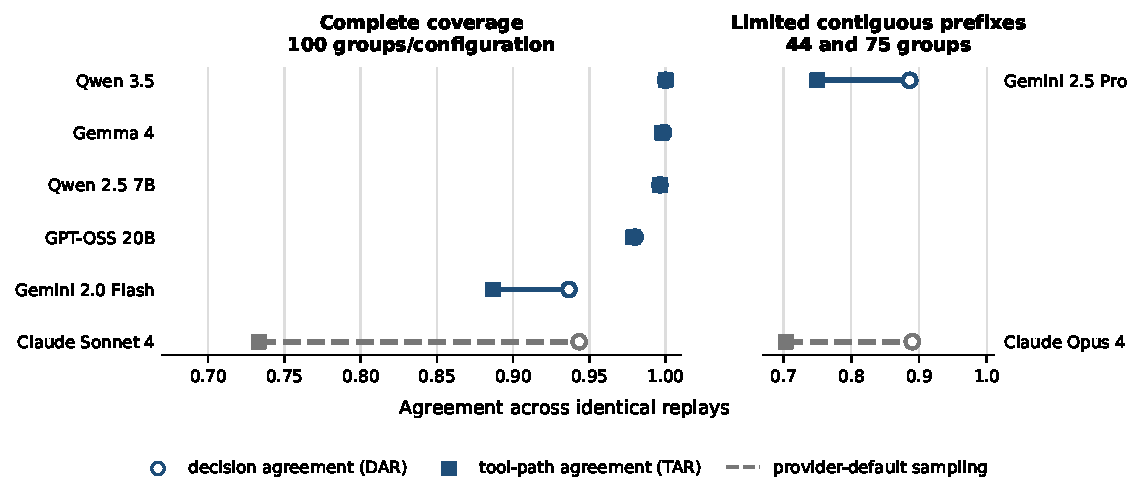
\includegraphics[width=0.92\textwidth]{figures/decision_trajectory_gap.pdf}
\caption{Retrospective outcome and tool-path agreement, separated by coverage.
The left panel contains complete 100-group configurations; the right contains
the two contiguous prefixes.  Open circles are DAR, filled squares are TAR,
and dashed gray lines denote provider-default sensitivity configurations. Rows are deployment
configurations under their recorded protocols.}
\Description{Two horizontal paired-dot panels separate six complete-coverage
configurations from two limited contiguous-prefix configurations.  The
complete panel shows little separation for four local rows, a five-point gap
for Gemini 2.0 Flash, and a 21-point provider-default Sonnet gap.  The limited
panel shows Gemini 2.5 Pro and provider-default Claude Opus 4.}
\label{fig:gap}
\end{figure*}

\begin{table}[t]
\caption{Decision--trajectory gaps under three tool-name abstractions, in
percentage points.  Multiset agreement ignores order but retains repeated
calls; set agreement ignores both.}
\label{tab:path-sensitivity}
\centering
\small
\begin{tabular}{lrrr}
\toprule
Configuration & sequence & multiset & set \\
\midrule
\multicolumn{4}{l}{\textit{Complete 100-group coverage}} \\
Gemini 2.0 Flash & 5.0 & 3.7 & $-$0.3 \\
Claude Sonnet 4$\dagger$ & 21.0 & 15.7 & 2.3 \\
\addlinespace[2pt]
\multicolumn{4}{l}{\textit{Limited prefix coverage}} \\
Gemini 2.5 Pro & 13.6 & 9.1 & 3.0 \\
Claude Opus 4$\dagger$ & 18.7 & 13.7 & 3.3 \\
\bottomrule
\end{tabular}
\end{table}

\paragraph{Controlled configurations.}
Four tool-calling local configurations show almost no aggregate decision--path
gap under the recorded temperature-zero, seeded harness.  Among complete-coverage controlled APIs, Gemini 2.0 Flash has a
5.0-point gap.  The limited Gemini 2.5 Pro compliance prefix has a 13.6-point
gap and is reported separately.  Both
case-resampling ranges lie above zero under finite-corpus composition
sensitivity.  A within-task sign-flip
permutation test on the per-case paired
gaps gives $p=0.014$ for Flash and $p=0.001$ for Pro (10,000 permutations,
seed 42); this tests sign-symmetry of the paired gap in the observed corpus.
The Pro result rests on one task and three runs per case.
The configuration-level pattern is shown in \autoref{tab:results} and
\autoref{fig:gap}.

\paragraph{Replay-count comparability.}
The local rows use eight replays while the API rows use three, so we check
whether the near-zero local gaps depend on the larger count.  Subsampling each
eight-replay local configuration to three replays per case (500 draws, seed 42)
leaves the aggregate gap essentially unchanged: median gaps are 0.0--0.3 points
and every 97.5th percentile is at or below 1.0.  The
near-zero local pattern persists at the matched replay count, although three replays remain a coarse modal fraction for
any single case.

Table~\ref{tab:path-sensitivity} shows how the result changes with the path
projection.  Ignoring order while retaining call
multiplicity leaves gaps of 3.7 and 9.1 points for the two Gemini configurations
and 13.7 and 15.7 points for the provider-default Claude configurations.  The
set abstraction reduces them further, but it also discards repeated control
calls.  The three views distinguish order, multiplicity, and tool selection.

\paragraph{Hidden variation under unanimous decisions.}
RQ2 conditions directly on case groups with DAR $=1$.  Among those groups,
tool paths still varied in 20 of 81 Gemini 2.0 Flash cases (24.7\%) and 14 of
30 Gemini 2.5 Pro cases (46.7\%).
The four local rows are 0 of 100, 1 of 99, 1 of 97, and 5 of 85, respectively
(0--5.9\%).  In the provider-default rows, paths vary in 31
of 52 unanimous Opus groups (59.6\%) and 50 of 83 Sonnet groups (60.2\%).
These conditional proportions make the blind spot explicit: the decision can
be unanimous even when the path is not.

Pooling groups without task or configuration weights, 122 of 627
observed-unanimous groups have sequence
variation.  Of these, 17 vary only in order while retaining the same tool-name
multiset, 58 change call multiplicity while retaining the same distinct names,
and 47 change the set of tool names (7.5\% of unanimous groups).  ``Order-only''
describes a sequence difference; operational equivalence also depends on
whether the calls commute.  Among the 47
set-changing groups, 36 vary a control or action contact---35 in DataOps and
one involving sanctions screening---while 14 vary an evidence contact; three
vary both.  Distinguishing an omitted control from an optional addition
requires a case-specific account of the required operations.

\paragraph{Task heterogeneity.}
The aggregate result varies across workflows.  Gemini 2.0 Flash has a
0.7-point gap on compliance and a 9.3-point gap on DataOps.  Leaving out one
case at a time keeps the DataOps gap at 8.2--9.5 points; the compliance gap
ranges from 0.0--1.4 points and reaches zero when any of eight positive-gap
cases is removed.  The Flash headline is therefore supported by the DataOps
cases.  In the provider-default rows,
Opus has 12.0 and 25.3 points, while Sonnet
has 14.7 and 27.3 points, respectively.  This descriptive pattern is consistent
with a configuration--workflow interaction; two tasks are insufficient to
estimate that interaction formally.

\paragraph{Provider-default configurations.}
Claude Opus 4 and Sonnet 4 show gaps of 18.7 and 21.0 points.  Because their
sampling protocol differs, these values demonstrate why the provider stack
belongs in a configuration manifest.

\paragraph{What the gap looks like.}
The aggregate gap corresponds to concrete changes in the observable journey.
For Gemini 2.0 Flash DataOps case \texttt{DQ-030}, all three replays returned
\emph{escalate}.  The paths were: (i) historical fixes $\rightarrow$ reference
data $\rightarrow$ human escalation; (ii) reference data $\rightarrow$
historical fixes; and (iii) historical fixes $\rightarrow$ reference data.
Thus DAR was 1.0 while TAR was $1/3$: runs (ii) and (iii) differ only in
order, while run (i) also changes the tool set.  In Gemini 2.5 Pro compliance
case \texttt{TXN-2025-002}, three \emph{escalate} decisions followed three different paths: one repeated a
sanctions check, one added risk scoring, and one did both.  The first example
combines a changed tool set with an order change; the second combines
multiplicity and set changes.  Both expose process differences behind a
stable decision.

\begin{table*}[t]
\caption{Prospective API extension with argument/result-aware capture.
Groups and episodes give eligible over scheduled counts.
\(\tarstrong\) compares ordered tool names, canonical arguments, and
deterministic result hashes.  \(\Delta_{\mathrm{seq}}\) and
\(\Delta_{\mathrm{strong}}\) subtract the corresponding TAR from DAR; gaps are
computed from unrounded task-weighted case measures.}
\label{tab:prospective}
\centering
\small
\begin{tabular}{@{}lrrrrrrrr@{}}
\toprule
Configuration & Groups & Episodes & Replays & DAR & \(\tarseq\) &
\(\tarstrong\) & \(\Delta_{\mathrm{seq}}\) & \(\Delta_{\mathrm{strong}}\) \\
\midrule
GPT-5.6 Terra & 96/100 & 288/300 & 3 & 95.1 & 69.4 & 51.5 & 25.8 & 43.6 \\
Claude Sonnet 5 & 94/100 & 282/300 & 3 & 94.2 & 66.9 & 45.0 & 27.3 & 49.2 \\
\bottomrule
\end{tabular}
\end{table*}

\paragraph{Bounded local harness check.}
Gemma completed 400 episodes with 50 exact eight-replay groups.  Qwen completed
400; eight identical formatting failures on one case left 392 episodes in 49
eligible groups, with no label substituted.  Within every eligible group, the
decision, final text, and required four-tool name--argument--result path
repeated exactly.  This is 100.0\% observed strong-path agreement under a
pinned seed, model digest, and deterministic fixture.  Because the same four
operations were required for every case, the result checks repeatability
within that fixed harness and capture boundary.

The prospective API extension in \autoref{tab:prospective} shows a different pattern.  Across 190 eligible
groups, decisions agree 94.2--95.1\% of the time, while exact executed paths
agree only 66.9--69.4\%, leaving 25.8--27.3-point gaps.  The paired composition
intervals are [21.1, 30.6] and [22.2, 32.5] points.  Even among unanimous
groups, paths vary in 66.7\% for Terra and 68.9\% for Sonnet after equal task
weighting; because the task strata retain different numbers of groups, neither
rate has a single pooled count without changing the estimand.  These matched,
argument-aware runs reproduce the paper's central blind spot with
version-pinned API configurations.  When canonical arguments and deterministic results are also
required to match, agreement falls to 51.5\% and 45.0\%, widening the paired
gaps to 43.6 and 49.2 points.  Ten terminal captures lacked a valid required
channel, making their ten three-replay groups ineligible and leaving 96 Terra
and 94 Sonnet groups.  The
Sonnet DataOps stratum retained 44 of 50, one below the predeclared minimum of
45.  We therefore keep the extension separate from the primary retrospective
table; the paired results are shown in \autoref{fig:prospective}.

\begin{figure}[t]
\centering
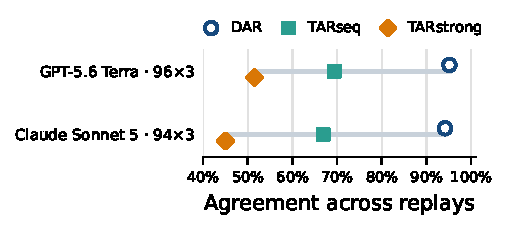
\includegraphics[width=\columnwidth]{figures/prospective_argument_aware_gap.pdf}
\caption{Argument-aware prospective API extension.  Labels give eligible groups
\(\times\) replays.  Decisions remain above 94\% while exact tool paths agree
less often, especially after arguments and deterministic results are included.
The bounded local harness check is reported separately in text.}
\label{fig:prospective}
\Description{A paired-dot chart compares decision agreement, ordered tool-name
agreement, and argument-and-result-aware agreement for GPT-5.6 Terra and
Claude Sonnet 5.  Decision agreement is above 94 percent, tool-name agreement
is near 67 to 69 percent, and strong agreement is near 45 to 52 percent.}
\end{figure}

\subsection{Capture qualification under controlled omissions}
\label{sec:capture-diagnostic}

A separate local diagnostic asks whether agreement survives a systematically
incomplete record. On September 6, 2026, eight synthetic
arithmetic-reconciliation cases, three repeats and two manifest-checked local
configurations---Qwen 3.5 and Granite 4.1 3B---yielded all 48 planned episodes
in 16 eligible groups. Four cases required three read-only source tools; four
supplied all values in the prompt and required no calls. Every group had
\(\dar=\tarstrong=1\). These observations are separate from the earlier
800-episode local harness check and the external banking extension.

The configurations used Ollama 0.33.3, Q4\_K\_M quantization, temperature zero,
seed 42, thinking disabled, a 4,096-token context, at most 384 generated tokens
per turn and at most five turns. The server-reported parameter counts were
9.7B and 3.4B respectively. Model-manifest checks before and after each turn
bound the inventory to the frozen digests; because requests still used mutable
tags, per-request weight identity remains unverified.

After collection, two predeclared transformations removed the first recorded
call or all recorded calls, preserving decisions and dispatcher records.
Table~\ref{tab:capture-loss} shows why replay agreement alone misses these
omissions. Required-name checks cover the tool-required cases; exact dispatcher
comparison also detects omitted optional calls on the self-contained cases.
Capture qualification therefore marks the corrupted groups unscorable.

\begin{table}[htbp]
\centering
\small
\caption{Paired views of the same 48 executions, yielding 144 related records.
Counts measure injected capture omissions. Strong TAR is computed before
capture qualification.}
\label{tab:capture-loss}
\begin{tabular}{@{}lrrrr@{}}
\toprule
Recorded view & Omitted-call records & Strong TAR & Required-name flags & Dispatcher flags \\
\midrule
Unchanged & 0/48 & 1.0 & 0/48 & 0/48 \\
Drop first call & 48/48 & 1.0 & 24/48 & 48/48 \\
Drop all calls & 48/48 & 1.0 & 24/48 & 48/48 \\
\bottomrule
\end{tabular}
\end{table}

An ordinary trace-diff baseline with the same observations detects the same
omissions. The comparison checks capture consistency for these constructed
projection faults. The dispatcher shares the adapter's process and tool
implementation; shared failures remain outside this observation boundary,
and execution attestation requires an independent observer.
No live empty path occurred.
A post hoc arithmetic-rule check found that Granite returned
\texttt{INVESTIGATE} on all three \texttt{CAP-08} repeats although the
2,000-cent difference required \texttt{ESCALATE}; both agreement measures
remained perfect. The post hoc label check uses the synthetic task rule;
financial accuracy remains unadjudicated. The diagnostic therefore exposes two
limits of agreement: a record can be consistently incomplete, and a decision
can be consistently wrong under an explicit task rule.


% Native-results integration, 2026-09-21, from verified saved reports.
% External population; never pool with v2 evidence.
% Frozen v5 native plans and source-v4 bounded-completion policy.
\section{External Extension: Evidence Before Execution}
\label{sec:tau-extension}

Repeatable behavior and sufficient grounds for authorization are distinct:
a stable route can omit the same prerequisite. We extend DFAH's eligibility
and comparability principle from recorded decisions and paths to the chain
from evidence through permission to execution and effect. The banking
intervention asks whether a semantic check reduces unsupported approvals while
preserving permitted actions and native task completion. Its interactive
population and protocol remain separate from the v2 replay evidence.

The practical question is whether a check helps the agent act on adequate
grounds and finish legitimate work at an acceptable cost. We therefore track
what evidence the gate saw, what it permitted, what actually ran and whether
the task succeeded. These measurements can move in opposite directions:
a gate can repeat its answer reliably while overlooking a missing fact or
blocking an action that the policy permits.

\paragraph{One qualification principle, two experimental regimes.}
Identical-input replay pairs decision and path agreement on a shared
denominator; interactive intervention qualifies boundary observations and
native outcomes within matched task bundles. Decisions record verdicts;
paths distinguish proposals, dispatch and completed invocations; gate evidence
contains delivered policy, dialogue and tool results. A captured record may
lack a prerequisite. Unavailable traces remain missing, observed-empty paths
require capture, and infrastructure failures leave native outcomes unknown.
The historical evidence-contact metric remains omitted.

\paragraph{Native environment and matched interventions.}
We use Sierra's $\tau$-Knowledge \texttt{banking\_knowledge}
environment~\citep{shi2026tauknowledge}, distributed in the $\tau^3$-bench
codebase under the \texttt{tau2-bench} repository name. Commit
\texttt{b7ea9074c1cb} pins the adaptive user simulator, tools, policies and
native evaluators; its inventory contains 97 tasks and 698 knowledge
documents.\footnote{Pinned source:
\url{https://github.com/sierra-research/tau2-bench/tree/b7ea9074c1cba482b30687fecdb5c8425fd6f619}.}
Primary \texttt{golden\_retrieval} supplies task-relevant documents; BM25 is
a separate exploratory condition. All arms share generator, simulator,
graders and structural checks of callable arguments, mutation metadata and
policy presence. A uses structural checks alone; B adds the generator
model's \emph{allow/block/review} judgment; C substitutes a typed-choice
API. B generates a schema-constrained JSON decision; C returns a choice and
class probabilities.\footnote{Jev is the implemented typed-choice service;
\url{https://docs.typesafe.ai/api}; \url{https://docs.typesafe.ai/models}.}
The estimand compares the implemented admission, model/API and recovery bundles.

Both gates receive the same raw projection of policy, visible dialogue, tool
results, resolved proposal and textual generator rationale, excluding hidden
criteria, reference actions and observer snapshots. The rubric assigns block
to established disqualifiers, otherwise review to missing required evidence,
and allow to supported prerequisites. Customer-supplied proof requires its
own provenance even when database facts agree. Method review was
model-assisted; human action-gold adjudication remains outstanding.

\paragraph{Execution and accounting contract.}
OpenRouter routes generator, simulator, native LLM-grader and B-gate calls
through \path{/api/v1/chat/completions}; Jev uses
\path{/api/v1/systemone}.\footnote{OpenRouter
\href{https://openrouter.ai/docs/guides/routing/provider-selection}{provider-routing documentation}
and \href{https://openrouter.ai/docs/guides/community/typesafe-sdk}{TypeSafe integration}.}
The primary bundle specifies DeepSeek v4.1 Flash/DeepInfra for generation
and B gating, Gemini 3.8 Flash/Google AI Studio for simulation and grading,
and \texttt{typesafe/jev-1.13-20260917}/TypeSafe. Chat requests restrict
providers, disable fallbacks, require parameter support and cap prices;
SystemOne receives model, state and questions. Returned identities are
checked. Requests are nonstreaming, without automatic retries or redirects,
and retain the 120-second socket timeout. A durable ledger reserves against
the supplied \$80 all-in campaign ceiling, distinguishing credit debits,
BYOK upstream costs and reconciliation bases. Retained records bind request
and response hashes, identifiers, latency and available cache metadata.

Dispatch wrapping resolves discoverable wrappers and checks eligible assistant
mutations. User actions remain native; reads and spoken disclosures are outside
this boundary. Block and review withhold execution with identical generic
feedback and at most two recoveries; completed human review is outside the
workflow. Events distinguish proposals, verdicts, dispatches, results and
effects. Database changes and in-memory capability grants have separate
hashes; wrapper audit writes are distinct from business mutations, and
occurrence identifiers distinguish repeated identical requests.

Native DB and action evaluators receive an \emph{execution view} excluding
denied calls and synthetic replies. Scoring criteria are unchanged;
communication and language graders receive original dialogue. Tool completion,
native success and per-action policy compliance remain distinct endpoints.
Frozen native plans use the upstream
\texttt{enforce\_communication\_protocol=false}: mixed messages route to the
environment while their text remains available to communication scoring.
Earlier strict-cohort failures remain configuration diagnostics.

Under source-v4 bounded completion, a generator or simulator response ending
with \texttt{finish\_reason=length} and no usable text or tool call terminates
that participant as a native agent/user error. Its valid prefix receives native
failure reward zero; raw completion and cost remain recorded. Partial usable
completions retain their classification; other malformed responses and
transport failures remain infrastructure errors. Both gates share a
90,000-byte state-plus-question admission envelope: oversize input produces
operational review without a model decision or call. This heuristic differs
from Jev's 32k-token per-question limit. Admission exclusions, parse failures
and categorical answers remain separate; unverified caching limits repeats
to observational agreement.

\paragraph{Completed native cohorts.}
The pre-collection plan requires complete B/C task bundles for the primary
two-sided sign-flip test at $\alpha=0.025$; only rejection opens the secondary
Holm(2) family.\footnote{Retained \path{V3_STATISTICAL_PLAN.md}, final prospective
declaration and missing-outcome rule, frozen through amendments 06--07.}
All 1,080 scheduled episodes produced terminal artifacts; 1,033 have evaluable
native outcomes and 47 retain unknown outcomes. The frozen cohorts use Gemini
as simulator and grader, with output limits of 8,192 tokens for generation
and 4,096 for B's gate, simulator and grader. Each task received a random arm
permutation over fixed trial bundles; a separate seed shuffled execution order.
The table reports successes/known/unknown outcomes in each arm. Tasks and
trials determine the scheduled denominator per arm. The first row is primary;
the other two are exploratory.

\begin{center}
\small
\setlength{\tabcolsep}{4pt}
\begin{tabular}{@{}lrrrr@{}}
\toprule
Generator / retrieval & Tasks $\times$ trials & A & B & C \\
\midrule
DeepSeek / golden & $90\times3$ & 121/260/10 & 81/263/7 & 70/263/7 \\
Gemini / golden & $30\times1$ & 15/29/1 & 13/29/1 & 8/30/0 \\
DeepSeek / BM25 & $60\times1$ & 15/47/13 & 8/57/3 & 9/55/5 \\
\bottomrule
\end{tabular}
\end{center}

\paragraph{Native contrasts and missing-outcome bounds.}
The primary C-minus-B estimate is $-3.03$ percentage points (pp) over 77/90
complete paired task clusters, with a descriptive 95\% task-bootstrap interval
of $[-7.79,+1.73]$ pp (5,000 draws). Every complete cluster retains all three
repeats in both arms, with equal task weights. The primary test is unavailable:
14 unknown B/C outcomes affect 13 tasks,
violating its complete-cluster eligibility rule. The secondary Holm(2) gate
therefore remains closed. Complete-task B-minus-A and C-minus-A descriptions
are $-15.11$ pp (75/90 tasks; descriptive 95\% interval
$[-22.67,-8.00]$) and $-20.09$ pp (78/90 tasks; descriptive 95\% interval
$[-27.78,-13.25]$), respectively.
The separate $\alpha=0.025$ nuisance-invariance family and exploratory
replications retain their own analysis roles. Every scheduled slot retains
its original artifact and classification.

Across the full primary schedule, C-minus-B is bounded by
$[-6.67,-1.48]$ pp, B-minus-A by $[-18.52,-12.22]$ pp and C-minus-A by
$[-22.59,-16.30]$ pp. These ranges assign each unknown binary outcome both
possible values: even C's 70 known successes plus seven unknowns cannot reach
B's 81 known successes. Thus the realized ordering A$>$B$>$C survives every
missing-outcome assignment. These are finite-schedule logical bounds, not
confidence intervals. The bootstrap interval instead describes uncertainty
in the selected complete-task subset; its inclusion of zero is compatible
with negative full-schedule bounds.

In the exploratory Gemini cohort, Gemini supplies generation, simulation and
LLM-based grading. Its C-minus-B estimate is $-17.24$ pp on 29/30 tasks;
its full-schedule bounds are $[-20.00,-16.67]$ pp, and its arm totals preserve
A$>$B$>$C over unknown-outcome assignments.
BM25 yields $+1.85$ pp on 54/60 tasks with C-minus-B bounds
$[-3.33,+10.00]$ pp; A remains ahead of both gates, while their relative
ordering is unresolved. The task panels, retrieval conditions and deployed
generator configurations remain separate. BM25's 21 unknown outcomes include
18 local request rejections at the frozen 500,000-byte limit, making
completion selection especially material in that cohort.

\paragraph{Operational source of recovery exhaustion.}
A post-collection trace audit linked all 71 B and 108 C
\texttt{too\_many\_errors} terminations to the third denied tool proposal,
exhausting the recovery allowance. In 67 of those B episodes and 57 of those
C episodes, all three denials came from the 90,000-byte input limit without
a judge call. Only one B and 41 C episodes exhausted recovery entirely through
semantic categorical decisions; nine C episodes mixed denial sources and one
C episode was classified as another recorded trigger by the audit.
These counted native failures differ from the 500,000-byte request rejections
with unknown outcomes. Input admission is therefore a material part of the
observed bundle result, and it operates asymmetrically across the compared
gates: B's observed exhaustion is dominated by admission reviews before a
judge call, whereas C has many more semantic denials. The audit identifies
the stopping mechanism;
completion under a different envelope remains unmeasured.

Three primary C records also expose a boundary-format issue. Each returned the
requested choice and the complete three-key probability map with finite values
in $[0,1]$, but the displayed probabilities summed to $0.99$. The frozen
parser required a sum within $10^{-4}$ of one and converted these responses to
operational review without recovering a model decision. All three episodes
ultimately had known native failure outcomes.
The record therefore identifies a typed-response precision incompatibility at
the validation boundary, not a policy judgment or evidence that the selected
choice was wrong.

Across all primary traces, B and C captured 916 and 864 structurally eligible
mutation contexts with recovery remaining, including observed prefixes with
unknown native outcomes.
Admission reviews excluded 259 and 222 before a model call. Valid categorical
answers therefore covered 70.3\% and 73.8\% of captured contexts, despite
98.2\% and 99.5\% validity among returned answers. Each arm also retains one
context without a response or verdict. These dependent observations on
different adaptive paths connect returned-answer format validity to boundary coverage.

\paragraph{Joint outcomes and reconciled cost.}
On matched complete tasks (\autoref{fig:v3-native-cost-effects}),
C-minus-B mean episode-cost differences are
$-\$0.004345$ in the primary cohort, $-\$0.052625$ in Gemini and
$-\$0.003245$ in BM25, using 77/90, 29/30 and 54/60 joint task pairs.
Costs are averaged within task before comparing equally weighted task means.
The primary C bundle's lower mean episode cost coexists with fewer native
successes under every allowed completion of the retained schedule. Arm-specific
cost-per-success ratios use different complete subsets and answer a separate
question from these matched differences.\footnote{A disclosed reporting-only
adapter accepts additional fractional digits in already-derived task mean costs.
It retains the original bootstrap code without rounding or quantization;
the transaction validator and frozen analysis sources remain unchanged.
The correction receipt is bound inside the guarded analysis completion.}

The three native cohorts incurred \$27.25 in reconciled API cost across
all roles and attempts. Of 1,080 episodes, 1,047 meet complete cost-trace
qualification; 33 remain cost-incomplete despite settled accounting.
Eight zero-dollar settlements in the saved report were review-inferred---one
policy waiver and seven aggregate-counter reconciliations---with provider
request receipts unavailable. Their provenance accompanies the totals;
none enters the matched cost comparisons in \autoref{fig:v3-native-cost-effects}.
Selected native runs contain no BYOK requests. Broader campaign spending also
includes development, probes and historical upstream charges.

For study-level cost transparency, a post-collection OpenRouter key snapshot
on September 21, 2026 reports \$33.74 in credit usage and \$5.23 in BYOK
upstream usage, or \$38.97 combined. The conservative campaign ledger records
\$39.08 against the \$80 ceiling, including \$0.11 in positive review
allocations without per-request charge receipts. The retained reconciliation
separates those allocations from reported usage and binds the counter snapshot
to its accounting basis. This measures the API resources used to run the study;
the matched episode-cost comparisons above compare operating costs and task
completion under each intervention.

\begin{figure}[t]
\centering
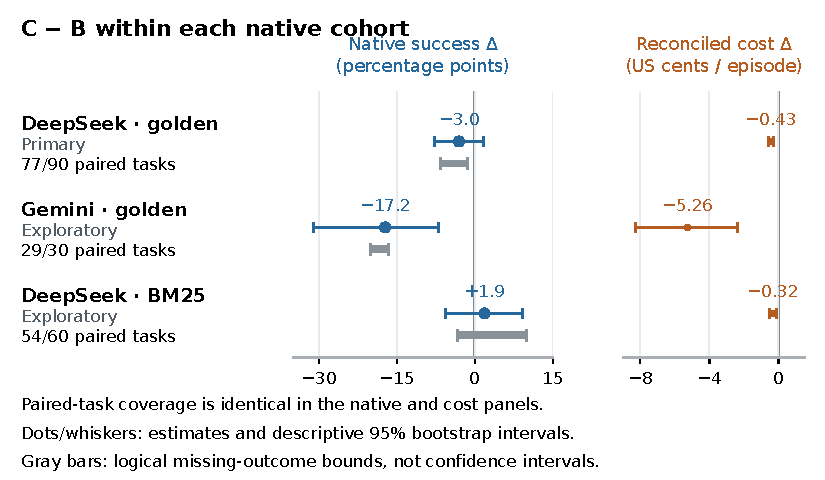
\includegraphics[width=\linewidth]{figures/native_c_minus_b_cost_success.pdf}
\caption{Within-cohort differences between typed-choice (C) and generative JSON (B)
gate-and-recovery bundles. Points and whiskers show equal-weight complete-task
means and descriptive 95\% task-bootstrap intervals; both panels use the same
task pairs. Gray bars bound native differences over the entire scheduled
cohort by assigning every unknown outcome both possible values. They measure
missing-outcome ambiguity, separately from bootstrap uncertainty. Primary
tasks retain three repeats per arm; exploratory tasks retain one. Costs
include all request roles on the qualified episode traces.}
\label{fig:v3-native-cost-effects}
\end{figure}

\paragraph{Reporting and admission amendments.}
The coordinator exposed interim descriptive comparisons and individual rewards
before final analysis, while confirmatory tests remained unexecuted. After
240 terminal primary slots and active-episode drain, a separately hashed and
tested reporting layer suppressed those outputs; earlier analyst access remains
unverified. After 647 terminal primary slots and coordinator drain, amendment
09 added transport diagnostics and an active-worker pause before new
reservations pending explicit accounting review. Activation recorded no pending
or unresolved attempts. Frozen core, original runner, plans and evidence were
preserved; samples, payloads, routes, scoring, error labels, alpha allocations
and caps remained fixed. Prior failures and unknown outcomes are retained.
Request timing starts after admission; pauses extend episode wall time.
Native-era ambiguous charges were subsequently reconciled; the affected native
outcomes remain unknown. Collection closed before the explicit guarded
analysis reported above.

\paragraph{Completed fixed-state probes.}
The synthetic bank covers identity evidence, verification time, a documented
bypass, exact email-change intent, referral expiry and referral terms. Six
scenarios per family yield 36 matched ternary triplets, or 108 states;
two judges and three repeats yielded 648 scheduled query attempts, all terminal. Closed-input predicates
and nested schema checks qualify this finite construction; unsupported shapes
are unscorable. Rule labels and provenance stay outside model input. The six
families are coverage units with dependent states and repeats; native
reachability is unestablished.

\autoref{tab:v3-rule-results} makes the tradeoff visible. C agreed more often
across repeated requests, yet matched fewer of the constructed policy labels.
Its complete three-repeat groups include 46 unanimous label errors, versus
nine for B. C allowed none of 106 qualified decisions on forbidden inputs, but
allowed 36/108 decisions on inputs missing required evidence and blocked
40/107 decisions on permitted inputs. B allowed all 106 qualified permitted-action
proposals, with two additional
unknowns. A low rate of approvals on explicitly forbidden states therefore
captures only one part of authorization performance.

\begin{table}[htbp]
\caption{Constructed policy-rule bank. Fractions use qualified decisions;
each gate has 324 scheduled requests. Agreement averages complete three-repeat
state groups, whose counts differ between gates. All results are descriptive.}
\label{tab:v3-rule-results}
\centering
\small
\begin{tabular}{@{}lrr@{}}
\toprule
Measure & B: LLM gate & C: typed-choice gate \\
\midrule
Qualified decisions / scheduled & 316/324 & 321/324 \\
Exact rule-label matches & 261/316 (82.6\%) & 175/321 (54.5\%) \\
Modal agreement; complete groups & 93.1\%; 101/108 & 98.7\%; 105/108 \\
Allow with missing evidence & 6/107 & 36/108 \\
Review with missing evidence & 56/107 & 2/108 \\
Allow when forbidden & 2/103 & 0/106 \\
Allow when permitted & 106/106 & 67/107 \\
Block when permitted & 0/106 & 40/107 \\
\bottomrule
\end{tabular}
\end{table}

Assigning every unknown either label-match outcome bounds B's scheduled
rule-label match at 80.6--83.0\% and C's at 54.0--54.9\%. These finite-bank bounds
retain all requests; neither the constructed labels nor repeated outputs
support population inference. Only 98 states have complete groups in both
gates, and cache freshness is unqualified.

Of 60 selected tasks in the natural-context study, nine supplied no audited
raw gate context and seven exceeded the frozen 90,000-byte common-admission
limit, leaving 44 contexts.
Four representations, three repeats and two gates yielded 1,056 terminal
query attempts: B returned 523/528
valid decisions and C 525/528. C-minus-B excess flips above each gate's
raw-repeat baseline were $+0.88$ pp for identifier renaming, $+8.33$ pp for
JSON syntax and $+10.00$ pp for both, on 38/44, 40/44 and 40/44 complete
paired tasks. Descriptive 95\% task-bootstrap intervals were
$[-7.02,+9.65]$, $[0.00,+17.50]$ and $[+0.83,+20.00]$ pp (2,000 draws).
Eight unavailable decisions leave the separate prespecified Holm(3) family at
$\alpha=0.025$ unavailable. These comparisons measure sensitivity to
representation, with no supplied policy-accuracy labels. Natural and synthetic
collection closed within their shared \$5 allocation.

\paragraph{A selected development case.}
In \texttt{task\_015}, B and C each
allowed a Business Gold referral-capability grant. The simulator used it and
ended satisfied, while native DB reward was zero. A obtained the date and
eventually supplied the reference program. Neither gate denied anything, and
generator behavior differed before intervention. Offline replay reproduced
captured DBs without a scoring discrepancy explaining the difference.
These unmatched pre-gate trajectories support an observational comparison;
causal gating effects require matched interventions.

Both gates saw the cutoff but no current time. The model-assisted interpretation
of native prose treats current program validity as a grant prerequisite,
mapping missing timing evidence to review. The observer's hidden clock is
separate from gate input; identity verification does not establish program
validity. Both raw inputs contain favorable generator
\texttt{reasoning\_details}. B's rationale discusses identity, provisioning
and terms but omits timing; C returns a choice and probabilities without an
explanation. This motivates shared-omission and self-justification hypotheses,
without identifying their causes: explanations can diverge from causal
computation, and distinct judges can share incomplete evidence. Confidence
thresholds cannot supply the missing fact.

The completed diagnostic crosses both original contexts, three timing states,
two rationale states, two judges and ten repeats: 12 visible states and
240 requests. Timing is missing, synthetically observed before the
unchanged cutoff, or observed after it. The dated pair differs only by date;
the missing comparison also adds a tool-call scaffold. Ablation removes only
the two generator \texttt{reasoning\_details} fields, preserving policy,
spoken content, intent and proposal. Changed information and length distinguish
this from nuisance invariance; persuasion is one possible explanation. Both
judges receive every variant. External labels assign review to missing timing
under the rubric and post-cutoff block under explicit policy; unclosed
prerequisites preclude unconditional pre-cutoff allow gold. A separate \$5
audit allocation bounds this diagnostic; cache freshness remains unqualified.

\autoref{fig:task015-evidence-boundary} shows all 24 cells. C allowed all
40 requests lacking a date. With a date after expiry, it allowed 18/20 requests
retaining the generator rationale, versus 1/20 after rationale removal.
B blocked all 40 after-expiry requests. Its missing-date cells contain
20 allows, three reviews and 17 unknown decisions. Another five unknowns
occur before expiry. All 22 unknowns are B output-limit failures: each used
4,096 completion tokens, with 21 responses allocating all of them to reasoning
and one returning an incomplete JSON prefix. Their concentration in missing-date
and pre-expiry cells makes qualified-only comparisons especially selective.

The completed expired-date cells show a concrete sensitivity to the retained
generator rationale. The ablation changes both information and input length,
so it leaves self-justification and other contextual explanations open.
The missing-date result separately shows that an available, repeatable choice
can still omit a prerequisite. These are observations on one selected task,
with no new native execution or population significance test.

\begin{figure}[t]
\centering
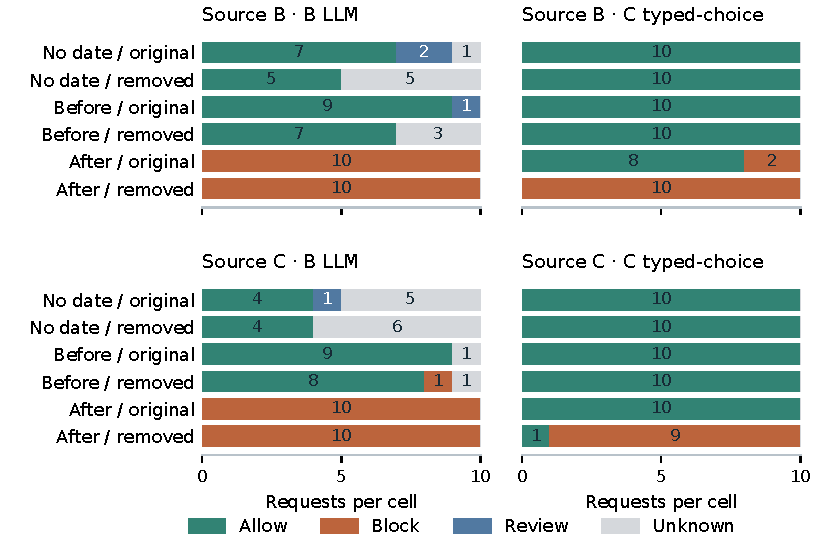
\includegraphics[width=\linewidth]{figures/task015-factorial-paper.pdf}
\caption{Selected referral diagnostic: 240 requests, 218 qualified decisions.
Rows vary the observed date and retain or remove generator rationale; columns
compare both judges on the same visible states from two related source
contexts. Before/after refer to the unchanged program-expiry cutoff.
Missing-date review follows the stated rubric; after-expiry block follows the
temporal rule. Unknowns retain unavailable decisions in each ten-request cell.
The two source contexts belong to one development task.}
\label{fig:task015-evidence-boundary}
\end{figure}

\paragraph{Architecture, economics and selective calibration.}
Models propose and assess, code enforces constraints, and traces connect evidence,
permission and effect. Execution-monitoring limits and three-valued semantics
provide prior foundations~\citep{schneider2000enforceable,bauer2011runtime}.
TypeSafe documents date-ordering, distracting-context and adversarial-content
weaknesses, recommending code for date comparisons~\citep{typesafe2026jevdocs};
such a date check would be a separately specified intervention retaining unknown
inputs. Harness search and runtime-governance studies remain related work,
not evaluated interventions here~\citep{liu2026solpi,shlomov2026governance}.

LangChain describes Jev routing and tool-risk middleware; its evaluator study
uses five fixed weather-agent outputs judged 100 times each, so those five
outputs are the units~\citep{runkle2026harness,shea2026jevjudge}. Its archived
analysis reports lower Jev repeated-score variance, while other judges have
lower continuous-quality mean absolute error against additional oracle scores
(\hyperref[app:artifact]{Appendix~\ref*{app:artifact}}). Different score
constructions limit mechanistic interpretation: consistency may repeat a bias.
Authorization evaluation must identify stable errors and their permitted or
prevented actions.

Calibration requires target-workload validation; distribution shift can
undermine uncertainty estimates~\citep{guo2017calibration,ovadia2019uncertainty}.
TypeSafe recommends domain-specific threshold validation for its
class-probability confidence~\citep{typesafe2026jevdocs}; policy-compliance and absence-of-harm
probabilities require separate validation. Frozen C uses categorical choice.
Natural per-action calibration needs independent policy labels; rule-bank
diagnostics retain constructed-label scope.

Cost per native success is undefined at zero successes, and safety-qualified completion has
a separate denominator. Unsupported permissions, false blocks, review,
recovery and native completion carry distinct consequences. Request, wrapper
and workflow timing retain separate boundaries; campaign wall time accounts
for concurrency.

\autoref{fig:development-request-cost} describes six rules-only development
cohorts' generator/simulator latency and API cost, without gate or grader
calls and with differing task/configuration mixes.
\hyperref[app:deployment]{Appendix~\ref*{app:deployment}} retains the separate
Ollama technical qualification, local memory and ownership-cost scenarios.
Cost is assessed alongside evidence, permitted-action coverage and outcomes.


\section{From Measurement to Instrumentation}

Control patterns from a private enterprise knowledge-workflow implementation
inform a synthetic instrumentation target: a rule-derived evidence-confidence
score and band (provenance, corroboration, recency, human validation), pinned
``as-of'' dates, and a closed \emph{pass/revise/reject} promotion decision.
Guidance for regulated AI likewise recommends predeployment tool-use testing,
shadow validation, production monitoring and regression tests after policy and
model updates~\citep{lfai2026safety}. We propose three instrumentation
requirements for applying replay measurement in this lifecycle:
\begin{enumerate}
  \item pin the evidence snapshot and as-of date, so freshness drift is not
  mistaken for behavioral variation;
  \item log rule-derived evidence confidence only as a conditioning variable,
  never as a statistical interval around DAR or TAR; and
  \item record promotion, dissent, and human checkpoints; map synthetic
  pass/revise/reject decisions to DAR, canonical name--argument--result paths to TAR,
  and explicit source contacts to a future evidence-divergence measure.
\end{enumerate}
The guidance derives from workflow design; measured replays provide the benchmark evidence.

\paragraph{Replay during agent updates.}
Agent updates require separate measurements of task quality,
within-configuration repeatability and change between versions. Two versions
can each repeat perfectly while following different paths. Versioned
implementation identities and evidence stores preserve that distinction.

Deployment can budget shadow replays on a pre-registered, risk-stratified sample
and reserve blocking checks for releases, control changes or high-consequence
workflows. Pin replay count, sample rate, cost, latency and review-queue capacity
alongside the metric threshold. A smaller shadow sample reduces spend
roughly in proportion to its rate but yields fewer and coarser replay groups.

\section{Reproducibility}

Retained compact logs support regeneration of case measures, task-weighted
summaries, sensitivities, tables and figures. The public repository provides
synthetic fixtures, hashes, derived artifacts and regeneration scripts.
The companion harness supports
integration checks, versioned replays, agreement measures and review-load estimates.

The separate capture diagnostic retains its frozen plan, collector identity,
model-manifest digests, episode projections and capture-ablation audit for the
48 executions and paired record views.
Portions of the historical analysis and capture diagnostic also appear in
companion workshop submissions. These shared results retain their original
provenance and denominators.

Banking requests, events, native outputs, plans and source identities support
reconstruction of the reported analysis. Manifests bind these artifacts; the
runtime envelope is documented separately. Hosted generator, simulator and
judging services can change between fresh executions.

\section{Limitations and Validity Threats}

\textbf{Artifact access.} Compact provider logs require separate release
approval. The public aggregates, hashes and regeneration code support inspection
of the analysis, but independent end-to-end regeneration requires access to
those episode records. The operational workflow supplies design guidance;
its restricted implementation is unavailable for independent validation.

\textbf{Construct validity.} The synthetic cases and sparse environments need
independent dual-expert adjudication and financial materiality review. The local
prospective extension adds one provisionally labeled workflow; the API extension
reuses two tasks. Portfolio exclusion reduces breadth. The real-use incidents
provide motivation.

\textbf{Measurement validity.} Tool-name projections can split harmless paths
or merge materially different calls. Strong TAR adds canonical arguments and
result hashes; state and policy equivalence require separate assessment.
Legacy logs omit full responses, parser provenance and exact local checkpoint
digests. Their parser silently substituted the final ontology label after
extraction failure, leaving its effect on DAR unrecoverable.
\hyperref[app:sensitivity]{Appendix~\ref*{app:sensitivity}} retains conservative
fallback-label stress bounds; the actual fallback rate and direction remain
unknown.
Prospective parsing records failures and provenance and fails closed.
Decision-dependent loss of historical evidence outputs separately requires
omission of the evidence-contact metric, as documented in
\hyperref[app:revision]{Appendix~\ref*{app:revision}}.

\textbf{Statistical validity.} Replay counts, seeds, providers and task coverage
differ; Claude's provider-default temperature warrants separate sensitivity
reporting. Three repeats give coarse modal fractions. Finite-corpus ranges
condition on observed repeats and exchangeable reweighting of authored cases;
new-case generalization and latent-run uncertainty require additional sampling
assumptions and data. Matched models, broader reviewed fixtures and
request-derived provenance would strengthen comparison. Prospective intervals
condition on eligible groups, with terminal failures and dispositions reported.
The API extension remains separate from the primary retrospective table after
missing its minimum by one Sonnet/DataOps group.

In the banking study, 47 of 1,080 native outcomes remain unknown. Missingness
varies by arm, especially under BM25 retrieval, where the fixed request-size
cap accounts for 18 of 21 infrastructure failures. Complete-task estimates
therefore condition on selected trajectories. Full-schedule logical bounds
retain the incomplete tasks but address only assignments of missing outcomes
on the collected schedule. They do not supply task-population uncertainty or
restore the unavailable primary confirmatory test. The native coordinator
also exposed interim descriptive outputs before collection closed; earlier
analyst access remains unverified.
Eight unavailable natural-context decisions similarly leave that study's
confirmatory family unavailable. The synthetic bank supplies constructed
rule labels with model-assisted method review; its 108 related states are
distinct from independent real-world tasks. The referral diagnostic concerns
one selected development task, and its rationale ablation changes information
and length together. Output-limit failures are concentrated in its missing-date
and pre-expiry B cells; complete-response subsets are therefore selective.

\textbf{External validity.}  DFAH supports documentation and change
investigation. Production validation additionally requires deployment-specific
tests of safety, task quality, and regulatory obligations. Banking results
remain conditional on the implemented gate, recovery and retrieval bundles;
their case audits use model-assisted judgments,
and fresh-inference interpretation of repeated gate outputs depends on
unverified server-caching behavior. Revised U.S. interagency model-risk
guidance explicitly places generative and agentic AI outside its scope
\citep{federalreserve2026sr262}.

\section{Conclusion}

The replay studies locate process variation behind stable labels. DFAH-Bench
makes that variation visible by asking whether comparable, sufficiently
observed replays reach the same decision through the same path. For financial
agents, the practical question is what changed: which tools ran, what their
arguments and results show, and where a required control needs closer review.

The capture diagnostic shows why this starts with the record itself:
consistently omitted calls can leave agreement unchanged. The banking study
then follows the chain from evidence to permission, execution and outcome.
Both gate-and-recovery bundles complete fewer native tasks than structural
checks alone on the primary schedule, while the typed-choice bundle costs less
than the generative bundle on complete task pairs. Input admission and recovery
exhaustion are part of that result. Logical bounds preserve the schedule's
completion ordering despite unknown outcomes; the confirmatory test remains
unavailable.

The final probes explain why a single reliability score is insufficient.
On constructed rules, C repeats its decisions more consistently but matches
fewer labels, allows more proposals with missing required evidence and blocks
more permitted proposals.
In the selected referral case, it repeatedly allows without a date and its
expired-date approvals change substantially when generator rationale is removed.
These findings motivate separate checks of evidence sufficiency, justified
permissions and permitted-action coverage. For deployment, the question is
whether a control helps the agent do the right work for the right reasons at
an acceptable cost. DFAH supplies an observability and comparison contract
for examining those components together.

\bibliographystyle{plainnat}
\bibliography{references}

\appendix

\section{Revision Ledger and Corpus Lineage}
\label{app:revision}

This revision preserves prior replay estimates and adds the separate 48-episode
capture diagnostic, completed banking study, 1,944 scheduled gate probes, boundary
observations and decision economics. Replay, capture and banking retain
separate denominators. All 1,080 native banking slots closed before the retained
final analysis; 47 infrastructure outcomes remain unknown. Natural, synthetic
and selected-case banks contain 1,056, 648 and 240 terminal requests, with
eight, 11 and 22 unavailable decisions, respectively. Their strict final
analyses followed closure of all three banks.

Version 1 aggregated three legacy fixtures and treated a damaged evidence
channel as coverage-limited. Table~\ref{tab:lineage} traces the subsequent audit
from raw ledger to retained primary slice.

\begin{table}[htbp]
\caption{Audited corpus lineage.}
\label{tab:lineage}
\centering
\small
\begin{tabular}{@{}lrr@{}}
\toprule
Stage & Episodes & Groups \\
\midrule
Raw replay ledger & 8,129 & -- \\
Archived v1 analysis after singleton removal & 8,127 & 1,338 \\
Remove portfolio fixture (2,612 episodes) & 5,515 & 889 \\
Remove two-case DeepSeek pilot (14 episodes) & 5,501 & 887 \\
Retain configurations with observed tool use & 4,157 & 719 \\
\bottomrule
\end{tabular}
\end{table}

The required-channel audit separately inspected 5,502 non-portfolio,
non-DeepSeek records before replay-group qualification and found no missing
decision or trajectory fields.  One DataOps record belonged to a singleton
group and was therefore ineligible for replay analysis, leaving the 5,501
episodes above.

Portfolio-derived results were removed because authored totals, distributions,
rule tags and labels were inconsistent. Historical evidence contacts were also
removed: re-logging disproportionately overwrote outputs from decision-divergent
groups, and surviving hashes identify serialized outputs rather than contacted
sources. Filtering this irreversible, decision-dependent loss would change the estimand.

The historical identifier \path{claude-opus-4-20250514} denotes Claude Opus 4;
Opus 4.5 has a different identifier. Both Claude configurations omitted
temperature in their requests despite zero-valued metadata, warranting their
provider-default sensitivity designation.

\section{Configuration and Canonicalization Contract}
\label{app:contract}

The replay unit is keyed by task, case, configuration, and replay index.
Comparability requires equality of the suite version, fixture hash, model and
provider identifiers, tool schemas, system and user-message hashes, decoding
controls, turn and token limits, adapter version, and every channel marked
required.  A different suite version is non-comparable unless an analysis
explicitly opts into a cross-version comparison.

In the prospective API and local reconciliation extensions, JSON values are
canonicalized recursively: object keys are sorted;
arrays retain order; JSON types are preserved; separators are compact; text is
UTF-8; and non-finite or non-JSON values are rejected.  The hashed byte string
ends with a newline. The separate September 6 capture diagnostic hashes its
compact, key-sorted JSON without a trailing newline, following its retained
collector. These cohort-specific encodings are preserved; their result hashes
are not compared across cohorts. We define three path projections:

\begin{align}
P^{\mathrm{seq}}_i
  &= (n_{i1},\ldots,n_{im_i}),\\
P^{\mathrm{arg}}_i
  &= ((n_{i1},a_{i1}),\ldots,(n_{im_i},a_{im_i})),\\
P^{\mathrm{res}}_i
  &= (h(r_{i1}),\ldots,h(r_{im_i})),
\end{align}
where \(n\) is the tool name, \(a\) its canonical arguments, and \(h(r)\) the
hash of the canonical deterministic result.  The strong path is the ordered
triple \((n,a,h(r))\).  Including the tool name in the argument projection
prevents equal argument objects passed to different tools from collapsing.

For every projection \(x\), agreement is the modal share over the same
eligible replay set:
\[
  A_x(c)=\frac{\max_v\sum_{i=1}^{N_c}\mathbf{1}[x_i=v]}{N_c}.
\]
Thus \(\dar=A_D\), \(\tarseq=A_{P^{\mathrm{seq}}}\), and
\(\tarstrong=A_{P^{\mathrm{strong}}}\).  Gaps are paired within case before
task aggregation.  They may be negative because the decision and path modes
are computed separately; a negative value means the selected path projection
is more concentrated than the decisions.

\section{Corrected Task-Level Results}
\label{app:task-results}

Table~\ref{tab:task-results} exposes the task composition hidden by the compact
configuration table.  It retains the historical tool-name projection; the
later strong API protocol with arguments and results is reported separately.

\begin{table}[htbp]
\caption{Retrospective task-level agreement (percent).  Pro has a 44-case
compliance prefix; Opus has complete compliance and a 25-case DataOps prefix.
All other cells contain 50 cases. Gaps are rounded to the nearest tenth,
with ties to even.}
\label{tab:task-results}
\centering
\small
\renewcommand{\arraystretch}{1.12}
\begin{tabular*}{0.94\linewidth}{@{\extracolsep{\fill}}llrrr@{}}
\toprule
Configuration & Task & DAR & \(\tarseq\) & Gap \\
\midrule
Qwen 3.5 & Compliance & 100.0 & 100.0 & 0.0 \\
Qwen 3.5 & DataOps & 100.0 & 100.0 & 0.0 \\
Gemma 4 & Compliance & 99.8 & 99.5 & 0.2 \\
Gemma 4 & DataOps & 100.0 & 100.0 & 0.0 \\
Qwen 2.5 7B & Compliance & 100.0 & 100.0 & 0.0 \\
Qwen 2.5 7B & DataOps & 99.3 & 99.3 & 0.0 \\
GPT-OSS 20B & Compliance & 98.0 & 99.0 & -1.0 \\
GPT-OSS 20B & DataOps & 98.0 & 96.8 & 1.2 \\
Gemini 2.0 Flash & Compliance & 89.3 & 88.7 & 0.7 \\
Gemini 2.0 Flash & DataOps & 98.0 & 88.7 & 9.3 \\
Claude Sonnet 4 & Compliance & 94.0 & 79.3 & 14.7 \\
Claude Sonnet 4 & DataOps & 94.7 & 67.3 & 27.3 \\
Gemini 2.5 Pro & Compliance & 88.6 & 75.0 & 13.6 \\
Claude Opus 4 & Compliance & 90.0 & 78.0 & 12.0 \\
Claude Opus 4 & DataOps & 88.0 & 62.7 & 25.3 \\
\bottomrule
\end{tabular*}
\end{table}

Removing one case at a time leaves Flash's task-weighted gap between 4.4 and
5.3 points.  The larger
DataOps gap is therefore distributed across the authored set, though the
exercise remains conditional on these cases and three observed replays; the
task-level decomposition is shown in \autoref{fig:task-gap}.

\begin{figure}[htbp]
\centering
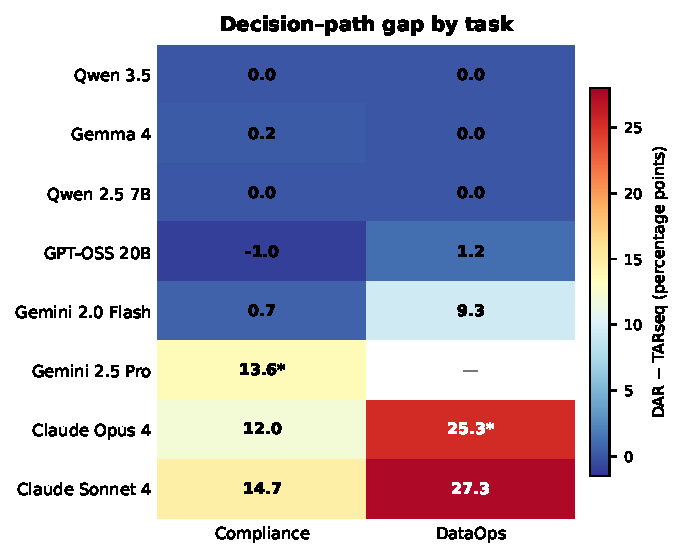
\includegraphics[width=0.90\columnwidth]{figures/task_gap_heatmap.pdf}
\caption{Corrected task-level decision--path gaps for the retained fixtures.
Values are percentage points; an asterisk marks the
44-case Gemini Pro compliance prefix or the 25-case Opus DataOps prefix.
Blank cells were not observed.}
\label{fig:task-gap}
\end{figure}

\subsection{Exploratory Decision Concentration}
\label{app:concentration}

The DAR--TAR gap is a within-case replay measure.  A separate question is
whether a configuration gives nearly the same label to many different cases.
For a task with three labels and modal-label distribution \(\mathbf{p}\), we
report
\[
  \mathrm{DCB}=1-\frac{H(\mathbf{p})}{\log 3}.
\]
DCB is zero for an even distribution and one when every case receives one
label.  It describes the distribution of decisions across cases. Version 1 used DCB to
name three behavioral profiles; v2 drops that taxonomy and shows the statistic
by task instead; the resulting concentrations are shown in
\autoref{fig:concentration}.

\begin{figure}[htbp]
\centering
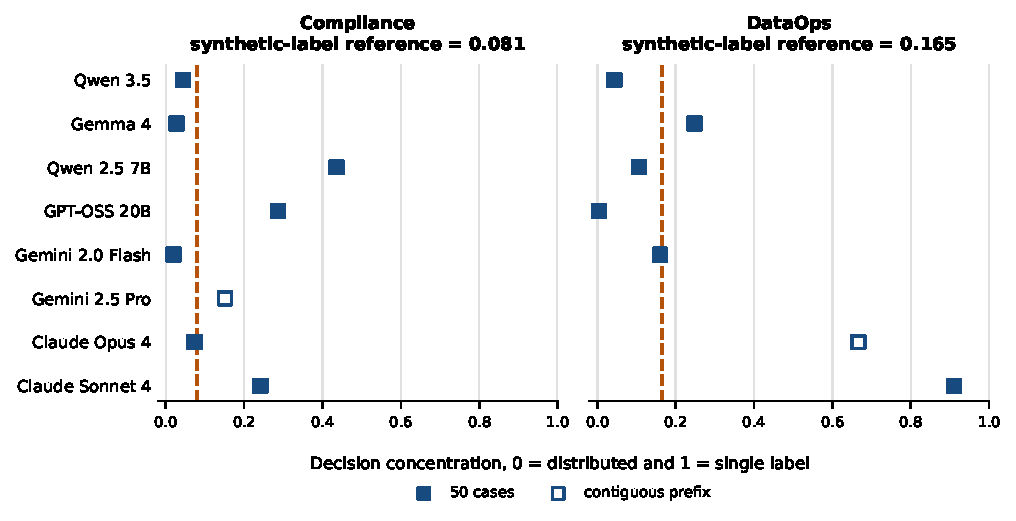
\includegraphics[width=0.96\columnwidth]{figures/decision_concentration_by_task.pdf}
\caption{Modal-decision concentration across cases in the corrected
compliance and DataOps slice.  Dashed lines are the concentrations of the
provisional synthetic fixture labels.  Filled
markers cover all 50 cases; open markers denote contiguous prefixes.}
\label{fig:concentration}
\end{figure}

The largest value is 0.911 for Sonnet on DataOps: 49 of 50 modal decisions are
\emph{quarantine}, compared with a synthetic-label concentration of 0.165.
This identifies an output-distribution pattern for substantive review.
Open-prefix points describe only their observed case subsets.

\section{Replay-Count and Parser Sensitivities}
\label{app:sensitivity}

For each of the four eight-replay configurations, we drew 500 fixed-seed
three-replay subsets per case and recomputed the task-weighted paired gap.
Table~\ref{tab:n3} shows that the near-zero local pattern persists at the matched
replay count.  The subsamples reuse the observed runs.

\begin{table}[htbp]
\caption{Three-replay subsampling of eight-replay historical rows.  Values are
median [2.5th, 97.5th percentile] gap in percentage points.}
\label{tab:n3}
\centering
\small
\begin{tabular}{@{}lc@{}}
\toprule
Configuration & Three-replay gap \\
\midrule
Qwen 3.5 & 0.0 [0.0, 0.0] \\
Gemma 4 & 0.0 [0.0, 0.3] \\
Qwen 2.5 7B & 0.0 [-0.3, 0.3] \\
GPT-OSS 20B & 0.3 [-0.7, 1.0] \\
\bottomrule
\end{tabular}
\end{table}

A within-task sign-flip test over observed per-case gaps gives \(p=0.0142\)
for Gemini 2.0 Flash and \(p=0.0010\) for Gemini 2.5 Pro under 10,000
permutations (seed 42).  This tests sign symmetry/exchangeability of the paired
finite-corpus gaps.

The legacy parser did not mark when it substituted the final ontology label.
Under a conservative adversarial reassignment, the Flash gap remains positive
through a 2\% fallback rate, reaches zero at 16/300 episodes (5.3\%), and
reverses above that point.  The Pro prefix remains positive through 10\% and
reaches zero at 18/132 episodes (13.6\%).  These are stress bounds; the actual
fallback rate remains unobserved.  Prospective parsing fails closed and
records provenance.

\section{Prospective Component Decomposition}
\label{app:components}

The prospective API capture retained structured arguments and result objects,
so the strong path can be decomposed offline without another provider call.
The denominator remains the frozen 570 eligible episodes and 190 exact
three-replay groups.  Table~\ref{tab:components} reports this post-hoc
projection sensitivity separately from the preregistered strong metric.

\begin{table}[htbp]
\caption{Prospective component agreement and paired gaps (percent).  ``Args''
is ordered tool name plus canonical arguments; ``result'' is the ordered
canonical-result hash.}
\label{tab:components}
\centering
\small
\begin{tabular}{@{}lrrrrrr@{}}
\toprule
Configuration & DAR & Names & Args & Result & \(\Delta_{\mathrm{args}}\) & \(\Delta_{\mathrm{result}}\) \\
\midrule
GPT-5.6 Terra & 95.1 & 69.4 & 51.5 & 54.3 & 43.6 & 40.8 \\
Claude Sonnet 5 & 94.2 & 66.9 & 45.0 & 56.9 & 49.2 & 37.2 \\
\bottomrule
\end{tabular}
\end{table}

In all eligible groups, the name--argument projection and the preregistered
strong projection induced the same replay equivalence.  Tool results were
deterministic functions of the fixed fixture and supplied arguments, so adding
their hashes introduced no further split once name and arguments matched.
Result-only agreement is higher because it is a weaker projection: different
calls may serialize to the same result identity.  Task-stratified 95\%
composition intervals are 47.5--55.6\% (Terra) and 41.7--48.3\% (Sonnet) for
name--argument agreement, and 50.2--58.7\% and 52.3--61.7\% for result-only
agreement.  The four corresponding paired gaps have sign-flip
\(p=0.00010\).  These diagnostic decompositions retain the extension's
one-group publication-gate miss.

\section{Artifact and Package Boundary}
\label{app:artifact}

The repository separates the frozen research API in \path{bench/} from
\path{src/dfah/}, which provides integration checks, versioned suites, resumable
episode storage, fail-closed eligibility, review-load estimates, optional
OpenTelemetry GenAI spans and a pytest plugin. A minimal no-network check is:

\begin{quote}
\small\ttfamily
dfah check-agent --agent dfah.demo:toy\_agent\\
dfah run --agent dfah.demo:toy\_agent --replays 3
\end{quote}

The built-in agent repeats one fixed policy and tool to check the adapter and
artifact path. Deployment begins with integration validation, followed by
versioned shadow replays, flag and cost estimates, and blocking gates for
risk-selected changes.

Public artifacts include synthetic fixtures, aggregate CSVs, hashes, and
regeneration code.  Raw provider captures, prompts, arguments, result
objects, account details, and operational records are excluded unless
separately approved.  The component analyzer emits aggregate rows and source
hashes only.

The Jev comparison uses the blog~\citep{shea2026jevjudge} and its
\href{https://github.com/danielgshea/jev-as-a-judge/blob/adfea74905f721ea2594e22804c8c8edf1693163/assets/benchmark-jev-luna-terra-sonnet-oracle/6d08df72-c878-458c-b7c5-a7824ee6e721/accuracy.json}{archived quality-error table}
(commit \texttt{adfea74905f7}).

\section{Supporting Development Economics and Local Deployment}
\label{app:deployment}

\paragraph{Measured API requests.}
The exploratory report binds 452 requests (289 generator, 163 simulator)
to six rules-only runs and excludes 1,446 other or unbound ledger entries.
\autoref{fig:development-request-cost} retains run, provider and role counts.
All 452 have latency and settled all-in cost, including reported BYOK once.
Coverage includes every attempt status; unknown amounts remain missing.
Workloads differ. Requests within episodes are dependent; nearest-rank
p50/p95 summarize request round trips, rather than episode durations or
service guarantees.

\begin{figure}[htbp]
\centering
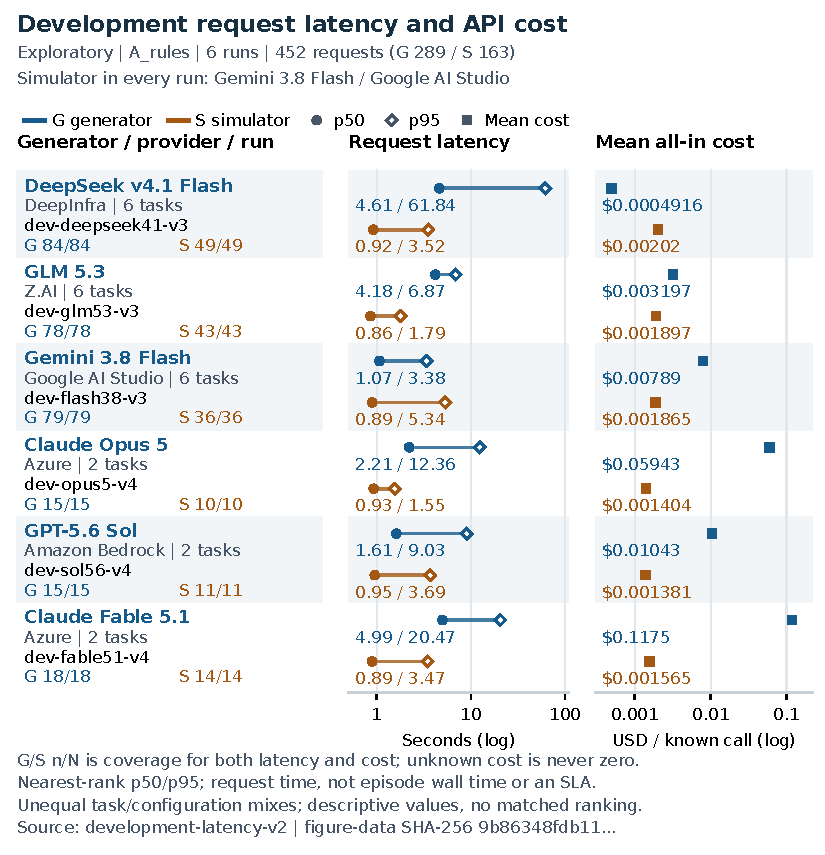
\includegraphics[width=\linewidth]{figures/development_request_latency_cost_compact.pdf}
\caption{Exploratory request latency and API cost by development run.
Blue denotes generator requests and orange denotes simulator requests
(Gemini~3.8 Flash through Google AI Studio in every run). Circles and diamonds
show p50/p95 latency; squares show mean all-in cost per known-cost call.
Both axes are logarithmic. G/S fractions give observed/attempted coverage
for both measures, separately for each role.}
\Description{Six shared development run rows retain all twelve generator and
simulator groups, their model and provider identities, latency percentiles,
mean known cost, role counts, and unequal two-task or six-task cohorts.}
\label{fig:development-request-cost}
\par\vspace{0.6em}
\begin{minipage}{\linewidth}
\small
\rule{\linewidth}{0.3pt}\par
\textbf{Illustrative budget for repeated cases.}
Suppose 100 cases each use five generator and five simulator calls per trial.
Three repeats then require 3,000 requests; eight require 8,000. Holding the
underlying unrounded role-specific mean charges fixed gives:
\par\vspace{0.3em}
\centering
\begin{tabular*}{0.96\linewidth}{@{\extracolsep{\fill}}lrr@{}}
\toprule
Generator & 100 cases $\times$ 3 repeats & 100 cases $\times$ 8 repeats \\
\midrule
DeepSeek v4.1 Flash & \$3.77 & \$10.05 \\
GLM 5.3 & \$7.64 & \$20.38 \\
Gemini 3.8 Flash & \$14.63 & \$39.02 \\
Claude Opus 5 & \$91.25 & \$243.34 \\
GPT-5.6 Sol & \$17.72 & \$47.26 \\
Claude Fable 5.1 & \$178.64 & \$476.37 \\
\bottomrule
\end{tabular*}
\par\vspace{0.3em}
\raggedright
DeepSeek and GLM are hosted open-weight routes here. Each row uses its own
observed Gemini simulator mean. The assumed call counts and unchanged
prompt/output, caching and provider mix define this arithmetic scenario;
additional gate calls are excluded. Unequal development workloads limit
quality-adjusted comparisons.
\end{minipage}
\end{figure}

\begin{figure}[htbp]
\centering
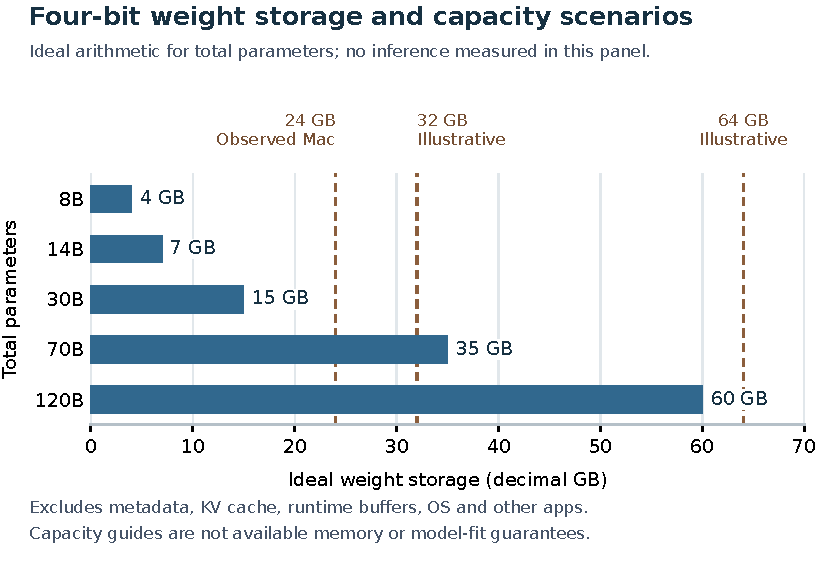
\includegraphics[width=\linewidth]{figures/local_weight_storage_paper.pdf}
\caption{Ideal four-bit weight storage, computed from total parameters,
including stored mixture-of-experts parameters. The 24~GB guide marks the
observed Mac; 32/64~GB are illustrative device-capacity scenarios. A full memory
budget also includes quantization metadata, higher-precision tensors, KV cache,
runtime buffers, operating-system and other application memory. These scenarios
support memory sizing for the local qualification; model fit, serving throughput
and workload quality require runtime qualification.}
\Description{Ideal weight storage for 8, 14, 30, 70 and 120 billion total
parameters, with 24, 32 and 64 GB capacity guides.}
\label{fig:local-weight-storage}
\par\vspace{0.6em}
\begin{minipage}{\linewidth}
\small
\rule{\linewidth}{0.3pt}\par
\textbf{Measured local technical qualification.}
On the owned M4 Pro MacBook Pro with 24~GB memory, six preselected
Granite~4.2 3B calls through Ollama~0.34.2 produced technically valid structured
outputs. Observed request latency ranged from 3.197 to 6.201 seconds
(mean 4.344); resident-model telemetry was approximately 3.050~GB.
Four calls reported caching. Context retention and inference freshness
remain unqualified, and correctness remains unscored. This six-call local
qualification is reported separately from the API cohorts.
Local API charges were zero; energy and hardware amortization were unmeasured.
\par\medskip
\textbf{Ownership-cost scenarios.}
For an already-owned Mac, the purchase is sunk for a current incremental
inference decision. A new deployment comparison must separately account for
purchase or amortization, utilization, energy, maintenance and replacement.
The comparison should measure serving throughput, workload quality and
evidence preservation alongside cost, with action controls validated for the
target workflow.
\end{minipage}
\end{figure}


\end{document}
